\chapter{Clasificación de los grupos de alumnos según su rendimiento}\label{sec:chapterXIII}
\addcontentsline{toc}{chapter}{Clasificación de los grupos de alumnos según su rendimiento}

Para realizar la identificación de los subconjuntos de alumnos definidos en la Sección \ref{sec:badstudents}, se empleará el algoritmo de clasificación de Quinlan C5.0 \cite{Quinlan:See5C5}, que no es más que una herramienta de aprendizaje supervisado que genera un árbol de decisión o un conjunto de reglas. Así pues, las distintas categorías en las que se clasificarán a los grupos vendrán dadas en las hojas de dichos árboles y en los consecuentes de las reglas respectivamente. El clasificador estadístico C5.0 se basa en el concepto de entropía, seleccionando primero aquellas características cuyos valores se diferencian más entre distintas categorías de grupos de alumnos.

Se utilizarán como variables de entrada del clasificador tanto las medidas clásicas de rendimiento presentadas en el Capítulo \ref{chapter:rendimiento} como las medidas grafo-teóricas (Sección \ref{sec:complexity}). Por su parte, como categorías de salida, tendremos tanto una única partición en alumnos ``LOW'', que se supone que requieren más esfuerzo para superar el laboratorio, como las cinco particiones que se muestran en la Figura \ref{fig:KMeans5}.

Dado que hay muy pocos registros ($77$ en cada nivel), el problema de clasificación va a ser difícil y, con el fin de aumentar las evidencias requeridas por C5.0 para trabajar, el conjunto de datos se agrupará cada tres niveles consecutivos. Así pues, por un lado, agruparemos los niveles $3$, $4$ y $5$ para realizar predicciones al principio de la práctica y, por otro lado, agruparemos los niveles $8$, $9$ y $10$. Así pues, las siguientes secciones se dividrán en dos subapartados, dependiendo de la parte del dataset que estemos utilizando para entrenar el clasificador.

\section{Clasificación empleando las métricas clásicas de rendimiento}



\section{Clasificación empleando las medidas de complejidad de propósito general}

\subsection{Clasificación empleando los niveles 3, 4 y 5}

El resultado es que C5.0 obtiene un conjunto de reglas capaz de clasificar exactamente los $35$ de los $36$ casos de grupos \emph{``LOW''} del nivel $3$ en adelante, es decir, a partir de un tercio del periodo de tiempo dedicado a la práctica, con un $p$ value $p = 3.843e-16$ estadísticamente muy relevante (Figura \ref{fig:cm2}). Además, las reglas obtenidas (Figura \ref{rules2}) tienen pleno sentido. Por ejemplo, la regla $7$ dice: ``Un grupo está en riesgo si está centrado en los problemas con numeración alta (\texttt{Be > 6})''. O la regla $3$ que dice ``Un grupo está en riesgo si no se ha centrado por igual en todos los problemas (\texttt{Ba > 3.366005}) y recorre caminos menos largos en media (\texttt{WDag > -4.317488}) teniendo en cuenta que el valor de máxima probabilidad de la métrica $WDag$ es $-4.19$.

\begin{figure}[H]
\centering
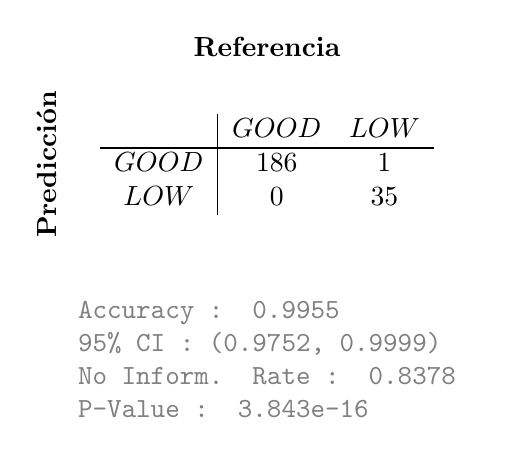
\begin{tikzpicture}
  \node (matrix)  {$\begin{array}{c|cc}
			 & GOOD & LOW \\ \hline
        GOOD & 186  & 1 \\
        LOW & 0 & 35
\end{array}$};
  \node[above of= matrix, node distance=0.5cm, yshift=1cm,font=\color{black}] {\textbf{Referencia}};
  \node[left of= matrix, node distance=3.5cm, rotate=90, anchor=center,yshift=-0.7cm,font=\color{black}] {\textbf{Predicción}};
  % Tabular environment for additional text
  \node[below of=matrix, node distance=2.5cm,font=\color{gray}]{
    \begin{tabular}{l}
      \texttt{Accuracy : 0.9955} \\
      \texttt{95\% CI : (0.9752, 0.9999)} \\
      \texttt{No Inform. Rate : 0.8378} \\
      \texttt{P-Value : 3.843e-16 }
    \end{tabular}
  };
\end{tikzpicture}
\caption{Aprendiendo a identificar a los grupos \emph{``LOW''}, es decir, aquellos con una puntuación inferior a $8.1$ sobre $10$.}
\label{fig:cm2}
\end{figure}

\begin{tcolorbox}[title=Reglas de clasificación para identificar grupos de tipo \emph{``LOW''}.]
  %add special color box to list of listings
  \makeatletter
  \addcontentsline{lol}{subsection}{\kvtcb@title}
  \makeatother
\begin{multicols}{2}
    \begin{minted}{R}
Rule 11/1: (17.8, lift 1.5)
	Ba > 9.26712
	->  class GOOD  [0.949]

Rule 11/2: (200.7/68.3, lift 1.0)
	De > 0.0952381
	->  class GOOD  [0.658]

Rule 11/3: (8.5/0.3, lift 2.5)
	WDag > -4.317488
	Ba > 3.366005
	->  class LOW  [0.880]

Rule 11/4: (5, lift 2.4)
	Dm <= 1.2
	Ef <= 4
	St > 1.791759
	->  class LOW  [0.858]

Rule 11/5: (8.3/0.6, lift 2.4)
	De <= 0.0989011
	Ef <= 4
	Ba <= 9.26712
	->  class LOW  [0.850]

Rule 11/6: (9.4/1.1, lift 2.3)
	De > 0.1153846
	Ef > 3
	Ef <= 4
	WDag <= -6.612041
	Ba > 3.366005
	->  class LOW  [0.818]

Rule 11/7: (3.4, lift 2.3)
	Be > 6
	->  class LOW  [0.814]

Rule 11/8: (13.3/2.3, lift 2.2)
	De <= 0.0952381
	Ba <= 9.26712
	->  class LOW  [0.783]

Rule 11/9: (19.9/5.4, lift 2.0)
	Dm <= 1.222222
	Ef <= 3
	St > 0.6931472
	Ba <= 9.26712
	->  class LOW  [0.707]
    \end{minted}
  \end{multicols}
\label{rules2}
\end{tcolorbox}

Pero no sólo esto, ¿podríamos dar un gran paso y predecir no sólo equipos \emph{``LOW''}/\emph{``GOOD''}, sino también un límite inferior y superior de sus calificaciones finales, y adivinar en cuál de los $5$ intervalos de la Figura \ref{fig:KMeans5} se encuentran? La respuesta es, felizmente, sí.

Efectivamente, C5.0 obtiene un conjunto de reglas (Figura \ref{rules5}) capaz de clasificar exactamente todos los grupos dentro de su correspondiente intervalo de calificaciones del nivel $3$ en adelante, es decir, a partir de un tercio del periodo de tiempo dedicado a la práctica, con un $p$ value $p < 2.2e-16$ estadísticamente muy relevante (Figura \ref{fig:cm5}).

\begin{figure}[H]
\centering
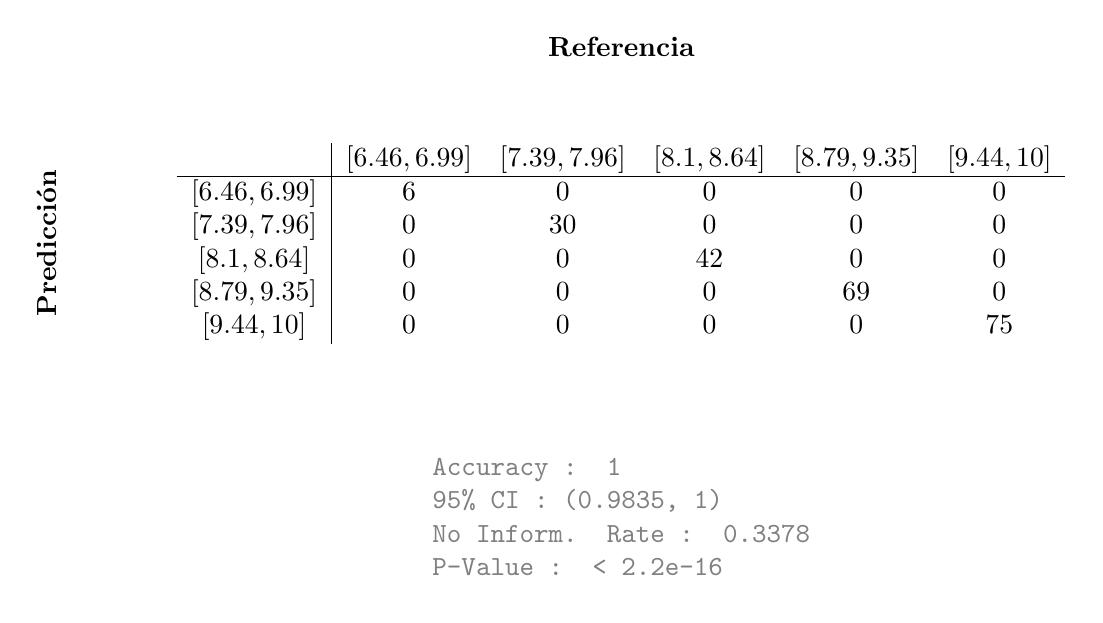
\begin{tikzpicture}
  \node (matrix)  {$\begin{array}{c|ccccc}
                         & \left[6.46,6.99\right] & \left[7.39,7.96\right] & \left[8.1,8.64\right] & \left[8.79,9.35\right] & \left[9.44,10\right]\\ \hline
        \left[6.46,6.99\right] & 6 & 0 & 0 & 0 & 0 \\
        \left[7.39,7.96\right] & 0 & 30 & 0 & 0 & 0 \\
        \left[8.1,8.64\right] & 0 & 0 & 42 & 0 & 0 \\
        \left[8.79,9.35\right] & 0 & 0 & 0 & 69 & 0 \\
        \left[9.44,10\right] & 0 & 0 & 0 & 0 & 75
\end{array}$};
  \node[above of= matrix, node distance=1.5cm, yshift=1cm,font=\color{black}] {\textbf{Referencia}};
  \node[left of= matrix, node distance=8cm, rotate=90, anchor=center,yshift=-0.7cm,font=\color{black}] {\textbf{Predicción}};
  % Tabular environment for additional text
  \node[below of=matrix, node distance=3.5cm,font=\color{gray}]{
    \begin{tabular}{l}
      \texttt{Accuracy : 1} \\
      \texttt{95\% CI : (0.9835, 1)} \\
      \texttt{No Inform. Rate : 0.3378} \\
      \texttt{P-Value : < 2.2e-16 }
    \end{tabular}
  };
\end{tikzpicture}
\caption{Aprendiendo a identificar a los grupos de prácticas con un intervalo de notas (Figura \ref{fig:KMeans5}).}
\label{fig:cm5}
\end{figure}

\begin{tcolorbox}[title=Reglas de clasificación para identificar intervalos de notas.]
  %add special color box to list of listings
  \makeatletter
  \addcontentsline{lol}{subsection}{\kvtcb@title}
  \makeatother
\begin{multicols}{3}
    \begin{minted}[fontsize=\scriptsize]{R}
Rule 99/1: (4.6, lift 4.7)
        We <= 0.01080108
        Ba > 3.366005
        ->  class [7.39,7.96]  [0.848]
Rule 99/2: (3.4, lift 4.5)
        We <= 0.2018018
        WDag <= -6.478509
        Be <= 1
        ->  class [7.39,7.96]  [0.815]
Rule 99/3: (9.4/2.2, lift 4.0)
        We <= 0.2702703
        St > 1.791759
        St <= 2.079442
        ->  class [7.39,7.96]  [0.721]
Rule 99/4: (11.1/3.5, lift 3.6)
        Cl > 0.2619048
        Di <= -4.219508
        We > 0.2131148
        We <= 0.2702703
        St > 0
        WDag <= -5.901418
      ->  class [7.39,7.96] [0.653]
Rule 99/5: (6.5/2.1, lift 3.5)
        De <= 0.0952381
        We <= 0.1321739
        ->  class [7.39,7.96]  [0.630]
Rule 99/6: (10.2/6.1, lift 2.3)
        St > 5.257495
        ->  class [7.39,7.96]  [0.414]
Rule 99/7: (7.6/0.5, lift 3.6)
        We > 0.2702703
        St <= 0
        WDag > -7.122867
      ->  class [8.1,8.64] [0.840]
Rule 99/8: (4.1, lift 3.6)
        We <= 0.2702703
        St > 2.079442
        WDag <= -5.296464
        Be <= 2
        ->  class [8.1,8.64]  [0.837]
Rule 99/9: (9.4/1.8, lift 3.2)
        Cl > 0.4095238
        We <= 0.2702703
        St > 0
        St <= 1.791759
        Dag > -5.204007
        Ba > 5.925958
        ->  class [8.1,8.64]  [0.751]
Rule 99/10: (6.3/1.9, lift 2.8)
        De <= 0.0952381
        We > 0.1321739
        ->  class [8.1,8.64]  [0.658]
Rule 99/11: (17.1/6, lift 2.7)
        De > 0.0952381
        We > 0.01080108
        We <= 0.04410441
        Ba > 3.366005
        ->  class [8.1,8.64]  [0.633]
Rule 99/12: (6.7/2.3, lift 2.7)
        We <= 0.01080108
        Ba <= 3.366005
        ->  class [8.1,8.64]  [0.621]   
Rule 99/13: (187.3/131.4, lift 1.1)
        We > 0.04410441
        ->  class [8.79,9.35]  [0.301]       
Rule 99/14: (9.2, lift 3.1)
        Cl > 0.2619048
        Di <= -4.219508
        We > 0.1415628
        We <= 0.2131148
        St > 0
        St <= 2.079442
        Ba <= 5.925958
        ->  class [9.44,10]  [0.911]
Rule 99/15: (7.1, lift 3.0)
        We > 0.2018018
        We <= 0.2287122
        St <= 0
        ->  class [9.44,10]  [0.890]
Rule 99/16: (6.8, lift 3.0)
        We > 0.2702703
        St <= 0
        WDag > -8.251143
        WDag <= -7.122867
        ->  class [9.44,10]  [0.886]
Rule 99/17: (5.5, lift 2.9)
        We > 0.2131148
        St <= 2.079442
        WDag > -5.901418
        ->  class [9.44,10]  [0.867]
Rule 99/18: (5.1, lift 2.9)
        We > 0.01080108
        We <= 0.04410441
        Ba <= 3.366005
        ->  class [9.44,10]  [0.860]
Rule 99/19: (4.7, lift 2.9)
        We > 0.04410441
        St <= 0
        WDag > -5.755742
        ->  class [9.44,10]  [0.851]
Rule 99/20: (11.5/1.3, lift 2.8)
        Dm <= 1
        Di <= -4.219508
        We > 0.04410441
        We <= 0.2131148
        St > 0
        Ba <= 5.925958
        ->  class [9.44,10]  [0.832]
Rule 99/21: (9.1/1.7, lift 2.6)
        Cl > 0.2792208
        We > 0.2702703
        St > 1.386294
        Dag > -5.204007
        Be > 1
        ->  class [9.44,10]  [0.759]
Rule 99/22: (10.6/2.6, lift 2.4)
        Cl <= 0.4095238
        De > 0.0952381
        St <= 1.791759
        Be > 2
        Ba > 5.925958
        ->  class [9.44,10]  [0.718]
    \end{minted}
  \end{multicols}
\label{rules5}
\end{tcolorbox}

\subsection{Clasificación empleando los niveles 8, 9 y 10}

El resultado es que C5.0 obtiene un conjunto de reglas capaz de clasificar exactamente los $36$ casos de grupos \emph{``LOW''} del nivel $8$ en adelante, es decir, a partir del último tercio del periodo de tiempo dedicado a la práctica, con un $p$ value $p < 2.2e-16$ estadísticamente muy relevante (Figura \ref{fig:cm3}). Además, las reglas obtenidas (Figura \ref{rules3}) tienen pleno sentido como en el caso anteriormente visto.

\begin{figure}[H]
\centering
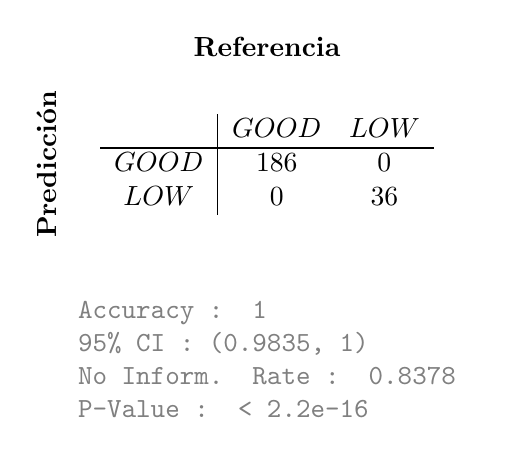
\begin{tikzpicture}
  \node (matrix)  {$\begin{array}{c|cc}
			 & GOOD & LOW \\ \hline
        GOOD & 186  & 0 \\
        LOW & 0 & 36
\end{array}$};
  \node[above of= matrix, node distance=0.5cm, yshift=1cm,font=\color{black}] {\textbf{Referencia}};
  \node[left of= matrix, node distance=3.5cm, rotate=90, anchor=center,yshift=-0.7cm,font=\color{black}] {\textbf{Predicción}};
  % Tabular environment for additional text
  \node[below of=matrix, node distance=2.5cm,font=\color{gray}]{
    \begin{tabular}{l}
      \texttt{Accuracy : 1} \\
      \texttt{95\% CI : (0.9835, 1)} \\
      \texttt{No Inform. Rate : 0.8378} \\
      \texttt{P-Value : < 2.2e-16}
    \end{tabular}
  };
\end{tikzpicture}
\caption{Aprendiendo a identificar a los grupos \emph{``LOW''}, es decir, aquellos con una puntuación inferior a $8.1$ sobre $10$.}
\label{fig:cm3}
\end{figure}

\begin{tcolorbox}[title=Reglas de clasificación para identificar grupos de tipo \emph{``LOW''}.]
  %add special color box to list of listings
  \makeatletter
  \addcontentsline{lol}{subsection}{\kvtcb@title}
  \makeatother
\begin{multicols}{2}
    \begin{minted}{R}
Rule 99/1: (8.3, lift 1.3)
	St <= 1.791759
	->  class GOOD  [0.903]

Rule 99/2: (8.3, lift 1.3)
	Be <= 1
	Ba <= 7.664816
	->  class GOOD  [0.903]

Rule 99/3: (81.3/11, lift 1.3)
	We > 0.4208696
	->  class GOOD  [0.855]

Rule 99/4: (72.7/13, lift 1.2)
	Cl <= 0.2771242
	We > 0.06390639
	We <= 0.4208696
	Be > 4
	->  class GOOD  [0.812]

Rule 99/5: (28.1/1.9, lift 2.8)
	We <= 0.4208696
	St > 1.791759
	Be <= 4
	Ba > 7.664816
	->  class LOW  [0.905]

Rule 99/6: (6.9, lift 2.7)
	Di > -8.386857
	St > 15.46906
	->  class LOW  [0.883]

Rule 99/7: (4.8, lift 2.6)
	Cl > 0.2771242
	Be > 4
	->  class LOW  [0.852]

Rule 99/8: (28.7/4.1, lift 2.6)
	We <= 0.4208696
	St > 1.791759
	Be > 1
	Be <= 4
	->  class LOW  [0.834]

Rule 99/9: (5.3/0.4, lift 2.5)
	We <= 0.06390639
	Be > 4
	->  class LOW  [0.815]
    \end{minted}
  \end{multicols}
\label{rules3}
\end{tcolorbox}

Adicionalmente, C5.0 obtiene un conjunto de reglas (Figura \ref{rules6}) capaz de clasificar exactamente todos los grupos dentro de su correspondiente intervalo de calificaciones del nivel $8$ en adelante, es decir, a partir del último tercio del periodo de tiempo dedicado a la práctica, con un $p$ value $p < 2.2e-16$ estadísticamente muy relevante (Figura \ref{fig:cm6}).

\begin{figure}[H]
\centering
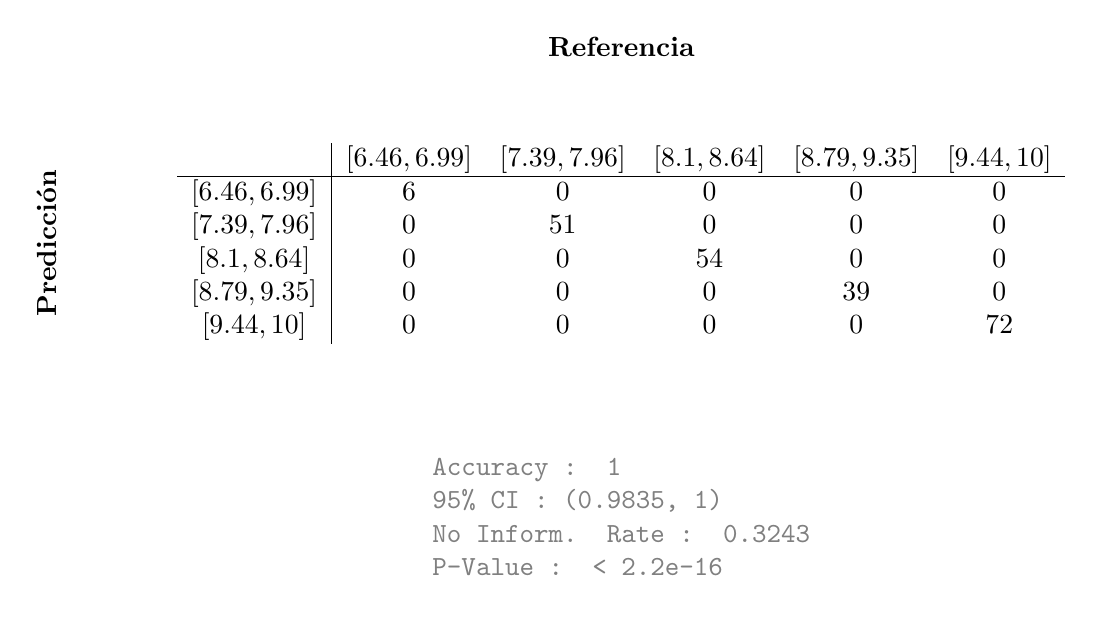
\begin{tikzpicture}
  \node (matrix)  {$\begin{array}{c|ccccc}
                         & \left[6.46,6.99\right] & \left[7.39,7.96\right] & \left[8.1,8.64\right] & \left[8.79,9.35\right] & \left[9.44,10\right]\\ \hline
        \left[6.46,6.99\right] & 6 & 0 & 0 & 0 & 0 \\
        \left[7.39,7.96\right] & 0 & 51 & 0 & 0 & 0 \\
        \left[8.1,8.64\right] & 0 & 0 & 54 & 0 & 0 \\
        \left[8.79,9.35\right] & 0 & 0 & 0 & 39 & 0 \\
        \left[9.44,10\right] & 0 & 0 & 0 & 0 & 72
\end{array}$};
  \node[above of= matrix, node distance=1.5cm, yshift=1cm,font=\color{black}] {\textbf{Referencia}};
  \node[left of= matrix, node distance=8cm, rotate=90, anchor=center,yshift=-0.7cm,font=\color{black}] {\textbf{Predicción}};
  % Tabular environment for additional text
  \node[below of=matrix, node distance=3.5cm,font=\color{gray}]{
    \begin{tabular}{l}
      \texttt{Accuracy : 1} \\
      \texttt{95\% CI : (0.9835, 1)} \\
      \texttt{No Inform. Rate : 0.3243} \\
      \texttt{P-Value : < 2.2e-16 }
    \end{tabular}
  };
\end{tikzpicture}
\caption{Aprendiendo a identificar a los grupos de prácticas con un intervalo de notas (Figura \ref{fig:KMeans5}).}
\label{fig:cm6}
\end{figure}

\begin{tcolorbox}[title=Reglas de clasificación para identificar intervalos de notas.]
  %add special color box to list of listings
  \makeatletter
  \addcontentsline{lol}{subsection}{\kvtcb@title}
  \makeatother
\begin{multicols}{3}
    \begin{minted}[fontsize=\scriptsize]{R}
Rule 99/1: (5.8, lift 24.4)
	De > 0.0992647
	We <= 0.2315271
	Dag <= -5.723585
	Ba > 6.816384
	->  class [6.46,6.99]  [0.871]

Rule 99/2: (8, lift 3.9)
	Dm > 2.666667
	Di > -8.386857
	Di <= -8.193677
	->  class [7.39,8.23]  [0.900]

Rule 99/3: (4.1, lift 3.7)
	De <= 0.1520468
	Dm > 2.666667
	->  class [7.39,8.23]  [0.837]

Rule 99/4: (5.7/0.3, lift 3.6)
	Cl > 0.2444444
	We > 0.409966
	Ba > 5.982207
	Ba <= 8.747471
	->  class [7.39,8.23]  [0.831]

Rule 99/5: (8/0.8, lift 3.6)
	Dm > 2.666667
	Di <= -8.193677
	We > 0.409966
	Dag > -5.834811
	WDag <= -2.246848
	->  class [7.39,8.23]  [0.822]

Rule 99/6: (7.9/1.4, lift 3.3)
	Cl > 0.2820513
	We <= 0.409966
	St > 1.098612
	->  class [7.39,8.23]  [0.759]

Rule 99/7: (4.7/0.9, lift 3.2)
	Cl <= 0.1421437
	Be <= 1
  ->  class [7.39,8.23] [0.723]

Rule 99/8: (71.1/45.1, lift 1.6)
	Dag <= -5.723585
	Ba > 6.816384
	->  class [7.39,8.23]  [0.369]

Rule 99/9: (7.9/0.5, lift 3.4)
	De > 0.1520468
	Di <= -8.386857
	We > 0.409966
	Dag <= -5.834811
	WDag <= -2.246848
	->  class [8.4,8.94]  [0.844]

Rule 99/10: (3.7, lift 3.4)
	Dm > 2.666667
	Di > -8.193677
	->  class [8.4,8.94]  [0.824]

Rule 99/11: (2.9, lift 3.3)
	Cl <= 0.2582892
	Di > -7.669682
	WDag > -4.185531
  ->  class [8.4,8.94] [0.796]

Rule 99/12: (8.7/1.2, lift 3.2)
	Cl <= 0.1728291
	We > 0.2315271
	We <= 0.409966
	Dag <= -5.723585
	Ba > 6.816384
	->  class [8.4,8.94]  [0.795]

Rule 99/13: (6/0.8, lift 3.2)
	Cl > 0.2582892
	Cl <= 0.2820513
	We <= 0.409966
	St > 1.098612
	Be <= 5
	->  class [8.4,8.94]  [0.772]

Rule 99/14: (8.4/3, lift 2.5)
	Ba <= 4.54026
	->  class [8.4,8.94]  [0.618]

Rule 99/15: (11.8/4.6, lift 2.4)
	Dm <= 2.666667
	Be <= 3
	Ba <= 5.982207
	->  class [8.4,8.94]  [0.592]

Rule 99/16: (31.7/18, lift 1.8)
	Dm <= 2.666667
	Dag > -5.834811
	Ba > 8.747471
	->  class [8.4,8.94]  [0.437]

Rule 99/17: (3.4, lift 3.5)
	We <= 0.409966
	Dag > -5.834811
	Dag <= -5.723585
	WDag <= -3.212575
	Ba <= 6.816384
  ->  class [8.98,9.44] [0.816]

Rule 99/18: (3.4, lift 3.5)
	Dm <= 2.666667
	We > 0.409966
	Dag <= -5.834811
	Ba > 8.747471
	->  class [8.98,9.44]  [0.815]

Rule 99/19: (27.8/4.5, lift 3.5)
	Cl <= 0.2582892
	Di > -7.669682
	We <= 0.409966
	St > 1.098612
	WDag > -6.650347
	WDag <= -4.185531
  ->  class [8.98,9.44] [0.815]

Rule 99/20: (6.9/1.3, lift 3.2)
	Cl <= 0.1421437
	Dm <= 2.666667
	We > 0.409966
	Be > 1
  ->  class [8.98,9.44] [0.748]

Rule 99/21: (18.7/6.1, lift 2.8)
	We <= 0.409966
	Dag <= -5.834811
	Ba <= 6.816384
  ->  class [8.98,9.44] [0.655]

Rule 99/22: (5.7, lift 3.4)
	Cl > 0.1705797
	Cl <= 0.2291667
	We > 0.409966
	Ef <= 8
	Ba > 8.747471
	->  class [9.54,10]  [0.870]

Rule 99/23: (4.7, lift 3.3)
	We <= 0.409966
	Dag > -5.834811
	WDag > -3.212575
	->  class [9.54,10]  [0.850]

Rule 99/24: (3.1, lift 3.1)
	Cl > 0.2582892
	Cl <= 0.2820513
	Be > 5
	->  class [9.54,10]  [0.803]

Rule 99/25: (5.3/0.6, lift 3.0)
	Le <= -8.4919
	Di <= -7.669682
	We <= 0.409966
	Dag > -5.723585
	->  class [9.54,10]  [0.775]

Rule 99/26: (9.3/3, lift 2.5)
	We <= 0.409966
	St <= 1.098612
	->  class [9.54,10]  [0.645]

Rule 99/27: (101.6/64.1, lift 1.4)
	We > 0.409966
	->  class [9.54,10]  [0.371]
    \end{minted}
  \end{multicols}
\label{rules6}
\end{tcolorbox}

\section{Clasificación empleando una combinación de todas las métricas}

A continuación, se repetirán los experimentos anteriores, pero ahora empleando las funciones $s$, $p$, $Cl$, $De$, $Dm$, $Le$, $Di$, $We$, $Ef$, $St$, $Dag$, $WDag$, $Be$ y $Ba$.

\subsection{Clasificación empleando los niveles 3, 4 y 5}

El resultado es que C5.0 obtiene un conjunto de reglas capaz de clasificar exactamente los $36$ casos de grupos \emph{``LOW''} del nivel $3$ en adelante, es decir, a partir de un tercio del periodo de tiempo dedicado a la práctica, con un $p$ value $p < 2.2e-16$ estadísticamente muy relevante (Figura \ref{fig:cm1}). Entre las reglas obtenidas (Figura \ref{rules1}), la regla $6$ dice: ``Un grupo está en riesgo si ha realizado pocas sesiones (\texttt{s <= 21}) y el grafo no está lo suficientemente balanceado (\texttt{Ba > 3,366005})''. O la regla $7$ que dice ``Un grupo está en riesgo si tiene pocas sesiones \texttt{We <= 0.01620162} y no se centra por igual en todos los problemas \texttt{Ba > 3.366005}''. %Esto es como el mal gráfico mostrado al principio de este documento en la Figura 1, largo y desconectado.

\begin{figure}[H]
\centering
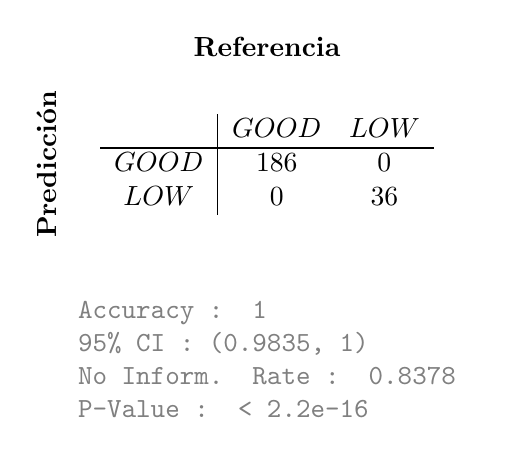
\begin{tikzpicture}
  \node (matrix)  {$\begin{array}{c|cc}
			 & GOOD & LOW \\ \hline
        GOOD & 186  & 0 \\
        LOW & 0 & 36
\end{array}$};
  \node[above of= matrix, node distance=0.5cm, yshift=1cm,font=\color{black}] {\textbf{Referencia}};
  \node[left of= matrix, node distance=3.5cm, rotate=90, anchor=center,yshift=-0.7cm,font=\color{black}] {\textbf{Predicción}};
  % Tabular environment for additional text
  \node[below of=matrix, node distance=2.5cm,font=\color{gray}]{
    \begin{tabular}{l}
      \texttt{Accuracy : 1} \\
      \texttt{95\% CI : (0.9835, 1)} \\
      \texttt{No Inform. Rate : 0.8378} \\
      \texttt{P-Value : < 2.2e-16}
    \end{tabular}
  };
\end{tikzpicture}
\caption{Aprendiendo a identificar a los grupos \emph{``LOW''}, es decir, aquellos con una puntuación inferior a $8.1$ sobre $10$.}
\label{fig:cm1}
\end{figure}

\begin{tcolorbox}[title=Reglas de clasificación para identificar grupos de tipo \emph{``LOW''}.]
  %add special color box to list of listings
  \makeatletter
  \addcontentsline{lol}{subsection}{\kvtcb@title}
  \makeatother
\begin{multicols}{2}
    \begin{minted}{R}
Rule 5/1: (20.9, lift 1.5)
	s > 177
	Ba <= 5.651057
	->  class GOOD  [0.956]

Rule 5/2: (21.2/0.3, lift 1.5)
	s > 21
	Cl > 0.6111111
	WDag > -6.562621
	->  class GOOD  [0.945]

Rule 5/3: (11, lift 1.4)
	Ba <= 3.366005
	->  class GOOD  [0.923]

Rule 5/4: (41.2/4.6, lift 1.4)
	WDag <= -6.678342
	->  class GOOD  [0.871]

Rule 5/5: (143.1/44.1, lift 1.1)
	Cl <= 0.4866667
	->  class GOOD  [0.689]

Rule 5/6: (12.4, lift 2.6)
	s <= 21
	Ba > 3.366005
	->  class LOW  [0.931]

Rule 5/7: (10.3, lift 2.6)
	We <= 0.01620162
	Ba > 3.366005
	->  class LOW  [0.918]

Rule 5/8: (19/1.4, lift 2.5)
	s > 177
	s <= 271
	Cl <= 0.4866667
	WDag > -6.39693
	Ba > 5.651057
	->  class LOW  [0.885]

Rule 5/9: (9.8/0.6, lift 2.4)
	s <= 105
	Cl <= 0.6111111
	We > 0.1657658
	->  class LOW  [0.868]

Rule 5/10: (19.6/4.3, lift 2.1)
	WDag > -6.678342
	WDag <= -6.562621
	->  class LOW  [0.755]

Rule 5/11: (26.4/7.8, lift 1.9)
	Cl > 0.4866667
	Cl <= 0.6111111
	WDag > -6.678342
	Ba > 3.366005
	->  class LOW  [0.690]
    \end{minted}
  \end{multicols}
\label{rules1}
\end{tcolorbox}

Igualmente, C5.0 obtiene un conjunto de reglas (Figura \ref{rules7}) capaz de clasificar exactamente todos los grupos dentro de su correspondiente intervalo de calificaciones del nivel $3$ al $5$, es decir, a partir del primer tercio del periodo de tiempo dedicado a la práctica, con un $p$ value $p < 2.2e-16$ estadísticamente muy relevante (Figura \ref{fig:cm7}).

\begin{figure}[H]
\centering
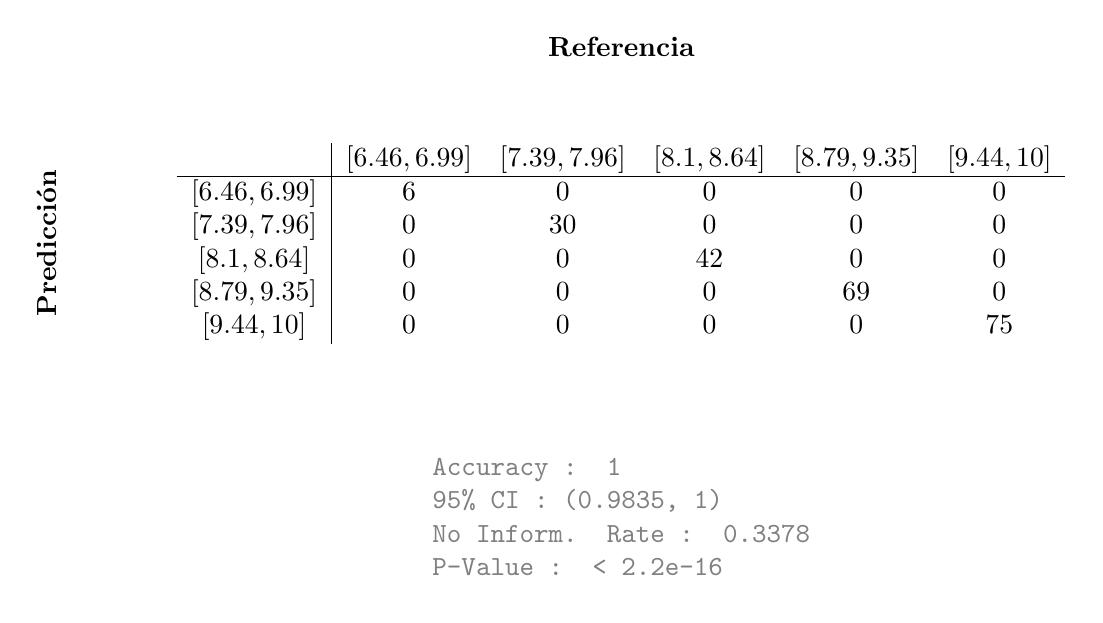
\begin{tikzpicture}
  \node (matrix)  {$\begin{array}{c|ccccc}
                         & \left[6.46,6.99\right] & \left[7.39,7.96\right] & \left[8.1,8.64\right] & \left[8.79,9.35\right] & \left[9.44,10\right]\\ \hline
        \left[6.46,6.99\right] & 6 & 0 & 0 & 0 & 0 \\
        \left[7.39,7.96\right] & 0 & 30 & 0 & 0 & 0 \\
        \left[8.1,8.64\right] & 0 & 0 & 42 & 0 & 0 \\
        \left[8.79,9.35\right] & 0 & 0 & 0 & 69 & 0 \\
        \left[9.44,10\right] & 0 & 0 & 0 & 0 & 75
\end{array}$};
  \node[above of= matrix, node distance=1.5cm, yshift=1cm,font=\color{black}] {\textbf{Referencia}};
  \node[left of= matrix, node distance=8cm, rotate=90, anchor=center,yshift=-0.7cm,font=\color{black}] {\textbf{Predicción}};
  % Tabular environment for additional text
  \node[below of=matrix, node distance=3.5cm,font=\color{gray}]{
    \begin{tabular}{l}
      \texttt{Accuracy : 1} \\
      \texttt{95\% CI : (0.9835, 1)} \\
      \texttt{No Inform. Rate : 0.3378} \\
      \texttt{P-Value : < 2.2e-16 }
    \end{tabular}
  };
\end{tikzpicture}
\caption{Aprendiendo a identificar a los grupos de prácticas con un intervalo de notas (Figura \ref{fig:KMeans5}).}
\label{fig:cm7}
\end{figure}

\begin{tcolorbox}[title=Reglas de clasificación para identificar intervalos de notas.]
  %add special color box to list of listings
  \makeatletter
  \addcontentsline{lol}{subsection}{\kvtcb@title}
  \makeatother
\begin{multicols}{3}
    \begin{minted}[fontsize=\scriptsize]{R}
Rule 99/1: (5.1/1.5, lift 19.5)
	Be > 3
	Ba > 7.831342
	->  class [6.46,6.99]  [0.646]

Rule 99/2: (6.7, lift 4.2)
	Cl <= 0.2380952
	St > 5.257495
	Ba <= 7.831342
  ->  class [7.39,7.96] [0.885]

Rule 99/3: (21.4/4.5, lift 3.7)
	s > 147
	We <= 0.2702703
	St <= 1.098612
	Ba <= 7.831342
	->  class [7.39,7.96]  [0.765]

Rule 99/4: (9.6/2, lift 3.5)
	s <= 21
	Ba > 3.291119
  ->  class [7.39,7.96] [0.742]

Rule 99/5: (5.6/1.2, lift 3.4)
	We <= 0.2702703
	St > 1.791759
	St <= 2.079442
	Ba <= 7.831342
	->  class [7.39,7.96]  [0.708]

Rule 99/6: (11/3.6, lift 3.1)
	s <= 146
	Le <= -6.421415
	St <= 2.079442
	->  class [7.39,7.96]  [0.646]

Rule 99/7: (6.4/0.4, lift 4.0)
	s > 150
	Cl > 0.1904762
	We <= 0.2702703
	St > 1.098612
	St <= 1.386294
	Ba <= 7.831342
	->  class [8.1,8.64]  [0.829]

Rule 99/8: (3.4, lift 4.0)
	Cl > 0.2380952
	St > 5.257495
  ->  class [8.1,8.64] [0.814]

Rule 99/9: (7.1/0.9, lift 3.8)
	Cl > 0.3583333
	We <= 0.2702703
	St > 2.079442
	->  class [8.1,8.64]  [0.790]

Rule 99/10: (2.4, lift 3.8)
	s > 146
	s <= 147
	Ba <= 7.831342
	->  class [8.1,8.64]  [0.773]

Rule 99/11: (8.7/2.5, lift 3.3)
	s > 21
	s <= 33
	->  class [8.1,8.64]  [0.670]

Rule 99/12: (8.4/3, lift 3.0)
	s > 33
	Cl <= 0.4222222
	We <= 0.07213115
	->  class [8.1,8.64]  [0.617]

Rule 99/13: (15.3/6.3, lift 2.8)
	We <= 0.4088335
	Be <= 3
	Ba > 7.831342
  ->  class [8.1,8.64] [0.579]

Rule 99/14: (4.4, lift 3.4)
	s <= 146
	p <= 5
	WDag <= -6.715384
  ->  class [8.79,9.35] [0.843]

Rule 99/15: (4, lift 3.4)
	s > 487
  ->  class [8.79,9.35] [0.833]

Rule 99/16: (11.5/1.4, lift 3.3)
	s <= 338
	We > 0.2702703
	St > 0
	St <= 5.257495
	Be <= 1
  ->  class [8.79,9.35] [0.823]

Rule 99/17: (3, lift 3.2)
	We > 0.4088335
	Ba > 7.831342
  ->  class [8.79,9.35] [0.802]

Rule 99/18: (2.5, lift 3.1)
	Cl <= 0.1904762
	St <= 5.257495
	Ba <= 7.831342
  ->  class [8.79,9.35] [0.778]

Rule 99/19: (17.4/5.9, lift 2.6)
	s <= 146
	p <= 5
	Le > -6.421415
	We > 0.07213115
	We <= 0.1805556
	St <= 2.079442
	Ba <= 7.831342
  ->  class [8.79,9.35] [0.643]

Rule 99/20: (199.9/135.5, lift 1.1)
	s > 33
	->  class [9.44,10]  [0.324]
    \end{minted}
  \end{multicols}
\label{rules7}
\end{tcolorbox}

\subsection{Clasificación empleando los niveles 8, 9 y 10}

El resultado es que C5.0 obtiene un conjunto de reglas capaz de clasificar exactamente los $36$ casos de grupos \emph{``LOW''} del nivel $8$ en adelante, es decir, a partir del último tercio del periodo de tiempo dedicado a la práctica, con un $p$ value $p < 2.2e-16$ estadísticamente muy relevante (Figura \ref{fig:cm4}). Las reglas obtenidas pueden consultarse en la Figura \ref{rules4}.

\begin{figure}[H]
\centering
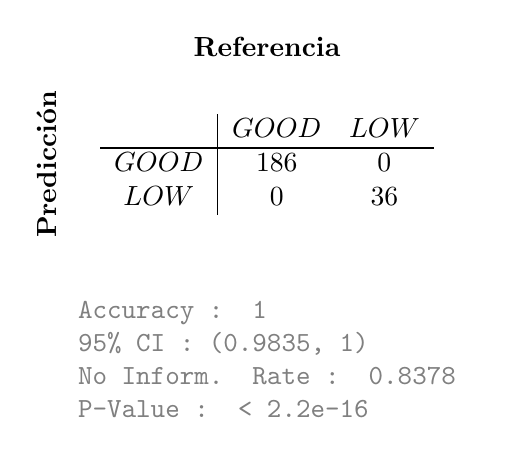
\begin{tikzpicture}
  \node (matrix)  {$\begin{array}{c|cc}
			 & GOOD & LOW \\ \hline
        GOOD & 186  & 0 \\
        LOW & 0 & 36
\end{array}$};
  \node[above of= matrix, node distance=0.5cm, yshift=1cm,font=\color{black}] {\textbf{Referencia}};
  \node[left of= matrix, node distance=3.5cm, rotate=90, anchor=center,yshift=-0.7cm,font=\color{black}] {\textbf{Predicción}};
  % Tabular environment for additional text
  \node[below of=matrix, node distance=2.5cm,font=\color{gray}]{
    \begin{tabular}{l}
      \texttt{Accuracy : 1} \\
      \texttt{95\% CI : (0.9835, 1)} \\
      \texttt{No Inform. Rate : 0.8378} \\
      \texttt{P-Value : < 2.2e-16}
    \end{tabular}
  };
\end{tikzpicture}
\caption{Aprendiendo a identificar a los grupos \emph{``LOW''}, es decir, aquellos con una puntuación inferior a una nota $8.1$ sobre $10$.}
\label{fig:cm4}
\end{figure}

\begin{tcolorbox}[title=Reglas de clasificación para identificar grupos de tipo \emph{``LOW''}.]
  %add special color box to list of listings
  \makeatletter
  \addcontentsline{lol}{subsection}{\kvtcb@title}
  \makeatother
\begin{multicols}{2}
    \begin{minted}{R}
Rule 11/1: (43, lift 1.6)
	p > 7
	We > 0.104152
	Ef <= 8
	St > 6.356108
	->  class GOOD  [0.978]

Rule 11/2: (32.2, lift 1.6)
	s > 443
	->  class GOOD  [0.971]

Rule 11/3: (24.2, lift 1.6)
	s > 187
	s <= 329
	p > 7
	St > 6.356108
	->  class GOOD  [0.962]

Rule 11/4: (24, lift 1.6)
	p > 7
	St > 6.356108
	Dag > -5.723585
	->  class GOOD  [0.962]

Rule 11/5: (24, lift 1.6)
	s <= 186
	We > 0.104152
	->  class GOOD  [0.961]

Rule 11/6: (23.7, lift 1.6)
	Cl > 0.1952381
	We > 0.104152
	St > 6.356108
	->  class GOOD  [0.961]

Rule 11/7: (20, lift 1.6)
	s > 187
	s <= 273
	p > 7
	Cl <= 0.2669468
	->  class GOOD  [0.955]

Rule 11/8: (18.6, lift 1.6)
	Cl <= 0.2669468
	We > 0.104152
	Dag > -5.480639
	->  class GOOD  [0.951]

Rule 11/9: (17.2, lift 1.6)
	Le > -8.653838
	We > 0.104152
	St > 6.356108
	->  class GOOD  [0.948]

Rule 11/10: (14.2, lift 1.5)
	Dm <= 1.142857
	->  class GOOD  [0.938]

Rule 11/11: (7.1, lift 1.5)
	Le <= -9.535989
	->  class GOOD  [0.890]

Rule 11/12: (28.6, lift 2.5)
	s > 329
	s <= 443
	Cl <= 0.1952381
	Le > -9.535989
	Le <= -8.653838
	Ef > 8
	Dag <= -5.723585
	->  class LOW  [0.967]

Rule 11/13: (18, lift 2.4)
	s > 273
	s <= 443
	Dm > 1.142857
	St <= 6.356108
	Dag <= -5.480639
	->  class LOW  [0.950]

Rule 11/14: (12.3, lift 2.4)
	s > 186
	s <= 187
	->  class LOW  [0.930]

Rule 11/15: (11.7, lift 2.4)
	Dm > 1.142857
	We <= 0.104152
	->  class LOW  [0.927]

Rule 11/16: (10.1, lift 2.4)
	s > 186
	p <= 7
	Dm > 1.142857
	->  class LOW  [0.917]

Rule 11/17: (10.1, lift 2.4)
	s > 186
	s <= 443
	Cl > 0.2669468
	Dm > 1.142857
	->  class LOW  [0.917]
    \end{minted}
  \end{multicols}
\label{rules4}
\end{tcolorbox}

Adicionalmente, C5.0 obtiene un conjunto de reglas (Figura \ref{rules8}) capaz de clasificar exactamente todos los grupos dentro de su correspondiente intervalo de calificaciones del nivel $8$ en adelante, es decir, a partir del último tercio del periodo de tiempo dedicado a la práctica, con un $p$ value $p < 2.2e-16$ estadísticamente muy relevante (Figura \ref{fig:cm8}).

\begin{figure}[H]
\centering
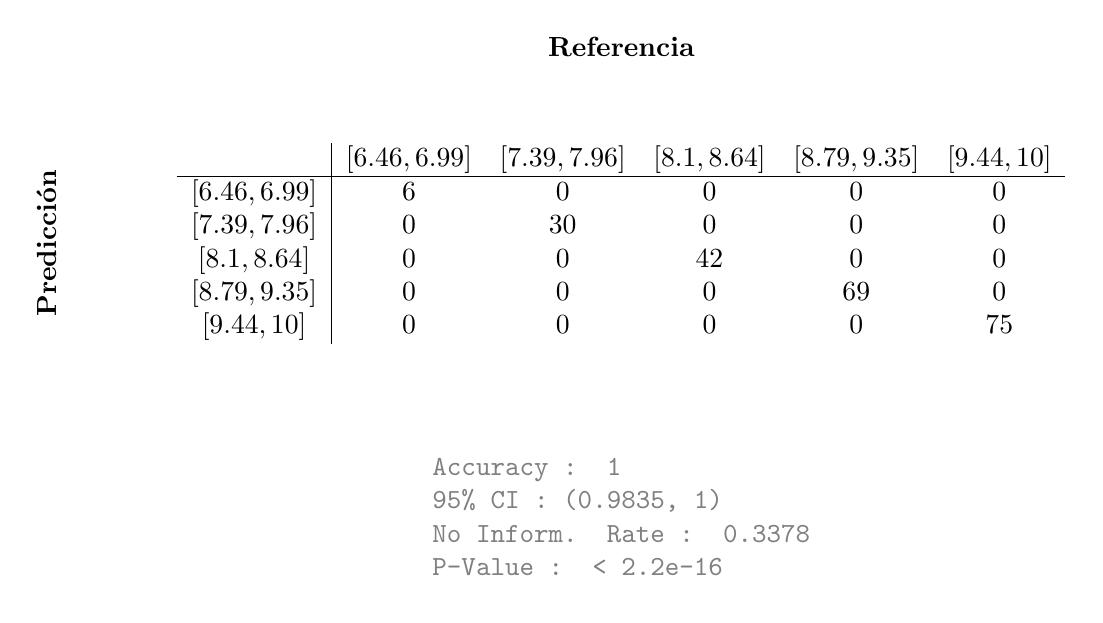
\begin{tikzpicture}
  \node (matrix)  {$\begin{array}{c|ccccc}
                         & \left[6.46,6.99\right] & \left[7.39,7.96\right] & \left[8.1,8.64\right] & \left[8.79,9.35\right] & \left[9.44,10\right]\\ \hline
        \left[6.46,6.99\right] & 6 & 0 & 0 & 0 & 0 \\
        \left[7.39,7.96\right] & 0 & 30 & 0 & 0 & 0 \\
        \left[8.1,8.64\right] & 0 & 0 & 42 & 0 & 0 \\
        \left[8.79,9.35\right] & 0 & 0 & 0 & 69 & 0 \\
        \left[9.44,10\right] & 0 & 0 & 0 & 0 & 75
\end{array}$};
  \node[above of= matrix, node distance=1.5cm, yshift=1cm,font=\color{black}] {\textbf{Referencia}};
  \node[left of= matrix, node distance=8cm, rotate=90, anchor=center,yshift=-0.7cm,font=\color{black}] {\textbf{Predicción}};
  % Tabular environment for additional text
  \node[below of=matrix, node distance=3.5cm,font=\color{gray}]{
    \begin{tabular}{l}
      \texttt{Accuracy : 1} \\
      \texttt{95\% CI : (0.9835, 1)} \\
      \texttt{No Inform. Rate : 0.3378} \\
      \texttt{P-Value : < 2.2e-16 }
    \end{tabular}
  };
\end{tikzpicture}
\caption{Aprendiendo a identificar a los grupos de prácticas con un intervalo de notas (Figura \ref{fig:KMeans5}).}
\label{fig:cm8}
\end{figure}

\begin{tcolorbox}[title=Reglas de clasificación para identificar intervalos de notas.]
  %add special color box to list of listings
  \makeatletter
  \addcontentsline{lol}{subsection}{\kvtcb@title}
  \makeatother
\begin{multicols}{3}
    \begin{minted}[fontsize=\scriptsize]{R}
Rule 99/1: (5.9, lift 18.9)
	p <= 8
	We <= 0.1196341
	->  class [6.46,6.99]  [0.873]

Rule 99/2: (8.4/4, lift 11.2)
	s > 384
	s <= 443
	p > 8
	Ba <= 7.57334
	->  class [6.46,6.99]  [0.519]

Rule 99/3: (4, lift 5.5)
	p > 8
	We <= 0.1196341
	St > 3.465736
	->  class [7.39,7.96]  [0.834]

Rule 99/4: (3.1, lift 5.3)
	s <= 384
	We > 0.1196341
	St > 1.098612
	Dag > -5.204007
	->  class [7.39,7.96]  [0.805]

Rule 99/5: (3.1, lift 5.3)
	s > 434
	s <= 443
	p > 8
	Ba > 7.57334
	->  class [7.39,7.96]  [0.803]

Rule 99/6: (2.7, lift 5.2)
	s <= 384
	Cl <= 0.1232493
	->  class [7.39,7.96]  [0.788]

Rule 99/7: (6.6/1.3, lift 4.8)
	s <= 282
	De <= 0.09356725
	We > 0.1196341
	Be > 5
	->  class [7.39,7.96]  [0.728]

Rule 99/8: (8.3/2.1, lift 4.6)
	s > 282
	s <= 384
	p > 8
	We > 0.1196341
	We <= 0.3631245
	St > 1.098612
	->  class [7.39,7.96]  [0.703]

Rule 99/9: (4.6, lift 4.4)
	s > 384
	s <= 443
	p <= 8
	->  class [8.1,8.64]  [0.848]

Rule 99/10: (4.1, lift 4.4)
	s <= 282
	WDag <= -7.014961
	->  class [8.1,8.64]  [0.836]

Rule 99/11: (11.2/1.5, lift 4.2)
	s > 443
	Cl <= 0.1833333
	We <= 0.4900901
	Dag <= -5.723585
	->  class [8.1,8.64]  [0.808]

Rule 99/12: (9.6/1.6, lift 4.1)
	s <= 282
	p > 8
	We > 0.1196341
	WDag <= -2.951776
	Be <= 2
	->  class [8.1,8.64]  [0.779]

Rule 99/13: (2.4, lift 4.0)
	s > 443
	Cl <= 0.1157051
	->  class [8.1,8.64]  [0.773]

Rule 99/14: (12.8/6.9, lift 2.4)
	p > 8
	We <= 0.1196341
	->  class [8.1,8.64]  [0.462]

Rule 99/15: (6.1, lift 3.0)
	s > 282
	s <= 443
	p <= 8
	Be <= 2
	->  class [8.79,9.35]  [0.876]

Rule 99/16: (203.4/138.5, lift 1.1)
	We > 0.1196341
	->  class [8.79,9.35]  [0.321]

Rule 99/17: (7.8, lift 2.8)
	s <= 282
	Dag > -5.834811
	WDag > -2.951776
	->  class [9.44,10]  [0.898]

Rule 99/18: (7, lift 2.8)
	s <= 384
	We > 0.1196341
	St <= 1.098612
	->  class [9.44,10]  [0.889]

Rule 99/19: (12.7/0.9, lift 2.7)
	s > 443
	Cl <= 0.1833333
	We > 0.4900901
	We <= 0.8403171
	Dag <= -5.723585
	Ba <= 8.747471
	->  class [9.44,10]  [0.874]

Rule 99/20: (16.7/6.1, lift 2.0)
	s > 443
	Cl > 0.1833333
	->  class [9.44,10]  [0.621]

Rule 99/21: (48.6/20.4, lift 1.8)
	s > 282
	s <= 384
	->  class [9.44,10]  [0.577]
    \end{minted}
  \end{multicols}
\label{rules8}
\end{tcolorbox}